\documentclass{tufte-handout}
%------------------------------------------------
%\geometry{showframe} % display margins for debugging page layout
%------------------------------------------------
\usepackage{graphicx} % allow embedded images
  \setkeys{Gin}{width=\linewidth,totalheight=\textheight,keepaspectratio}
  \graphicspath{{/home/swl/Dropbox/ucd/eu_economics/figs/}}  % set of paths to search for images
\usepackage{amsmath}  % extended mathematics
\usepackage{booktabs} % book-quality tables
\usepackage{units}    % non-stacked fractions and better unit spacing
\usepackage{multicol} % multiple column layout facilities
\usepackage{lipsum}   % filler text
\usepackage{fancyvrb} % extended verbatim environments
  \fvset{fontsize=\normalsize}% default font size for fancy-verbatim environments

%------------------------------------------------
% Standardize command font styles and environments
\newcommand{\doccmd}[1]{\texttt{\textbackslash#1}}% command name -- adds backslash automatically
\newcommand{\docopt}[1]{\ensuremath{\langle}\textrm{\textit{#1}}\ensuremath{\rangle}}% optional command argument
\newcommand{\docarg}[1]{\textrm{\textit{#1}}}% (required) command argument
\newcommand{\docenv}[1]{\textsf{#1}}% environment name
\newcommand{\docpkg}[1]{\texttt{#1}}% package name
\newcommand{\doccls}[1]{\texttt{#1}}% document class name
\newcommand{\docclsopt}[1]{\texttt{#1}}% document class option name
\newenvironment{docspec}{\begin{quote}\noindent}{\end{quote}}% command specification environment
%------------------------------------------------

%------------------------------------------------
%%%% Details %%%%
%------------------------------------------------
\title{European Economy: Fiscal policy}
\author{University College Dublin}
\date{Spring 2017} 

\begin{document}
\maketitle  
%------------------------------------------------------------------------------
%%%% Fiscal policy %%%%
\section{Fiscal policy basics}
When countries join a monetary union they give up on one of their macroeconomics instruments namely monetary policy. 
But they retain autonomy over setting fiscal policy. 
Therefore in a monetary union fiscal policy will be the only instrument the government can use to deal with asymmetric shocks.
Unfortunately, fiscal policy is not really a good alternative to monetary policy for two main reasons
\begin{enumerate}
  \item The budget needs to be balanced
  \begin{itemize}
    \item Consider the case where a government wants to increase private spending by cutting taxes
    \item This will create a budget deficit which needs to be accounted for, so the government borrows
    \item Borrowing of course will lead to a debt which needs to be paid off, likely through a future tax increase\marginnote{Undisciplined fiscal policy can lead to high levels of public indebtedness.}
  \end{itemize}
  \item It is slow to implement
  \begin{itemize}
    \item Establishing the budget is a long political process
  \end{itemize}
\end{enumerate}
\marginnote{Note that counter-cyclical fiscal policies can be effective as the government, when deemed credit worthy, can borrow money more easily compared to firms and households. Also note that in an optimum currency area, in lieu of actual transfers, a country hit by a shock could borrow money from a country unaffected by the shock.}

One important factor of fiscal policy is that it tends to be counter-cyclical, meaning that when the economy slows down tax revenue will decline and spending on unemployment benefits will increase. 
If the budget worsens, fiscal policy will automatically be expansionary: one average a 1\% decrease in economic growth corresponds to a 0.5\% deterioration in the budget balance relative to GDP.\footnote{Note that there are of course differences across countries, depending on the tax and welfare system.} 
These features of the government budget, which help dampen the impact of fluctuations in the business cycle, are known as automatic stabilizers. 
In contrast to automatic stabilizers there is also discretionary policy actions, where the government takes active action. 
Since, as discussed, taking these kind of actions might be slow, most countries tend to keep some budget on the side as a sort of rainy day fund to use when the economy contracts. 
Note that the budget figures might obscure what the government is actually doing with its fiscal policy as the budget can change for two reasons
\begin{enumerate}
  \item Discretionary policy action; the budget can improve due to spending cuts or increased taxes
  \item Automatic stabilizers; the budget improves due to the fact that the economy is in a boom state
\end{enumerate}

To disentangle these two factors we therefore use the cyclically-adjusted budget balance, which relies on the output gap to measure the performance of the economy relative to its potential output. 
The difference between the measured budget balance and the cyclically-adjusted budget balance is the work of the automatic stabilizers. 
Figure~\ref{fig:rabo} shows this for the Netherlands, it illustrates that in general the budget balance moves in tandem with the output gap, which indicates the effect of the automatic stabilizers. 

%--------------------------------------
\begin{figure}
  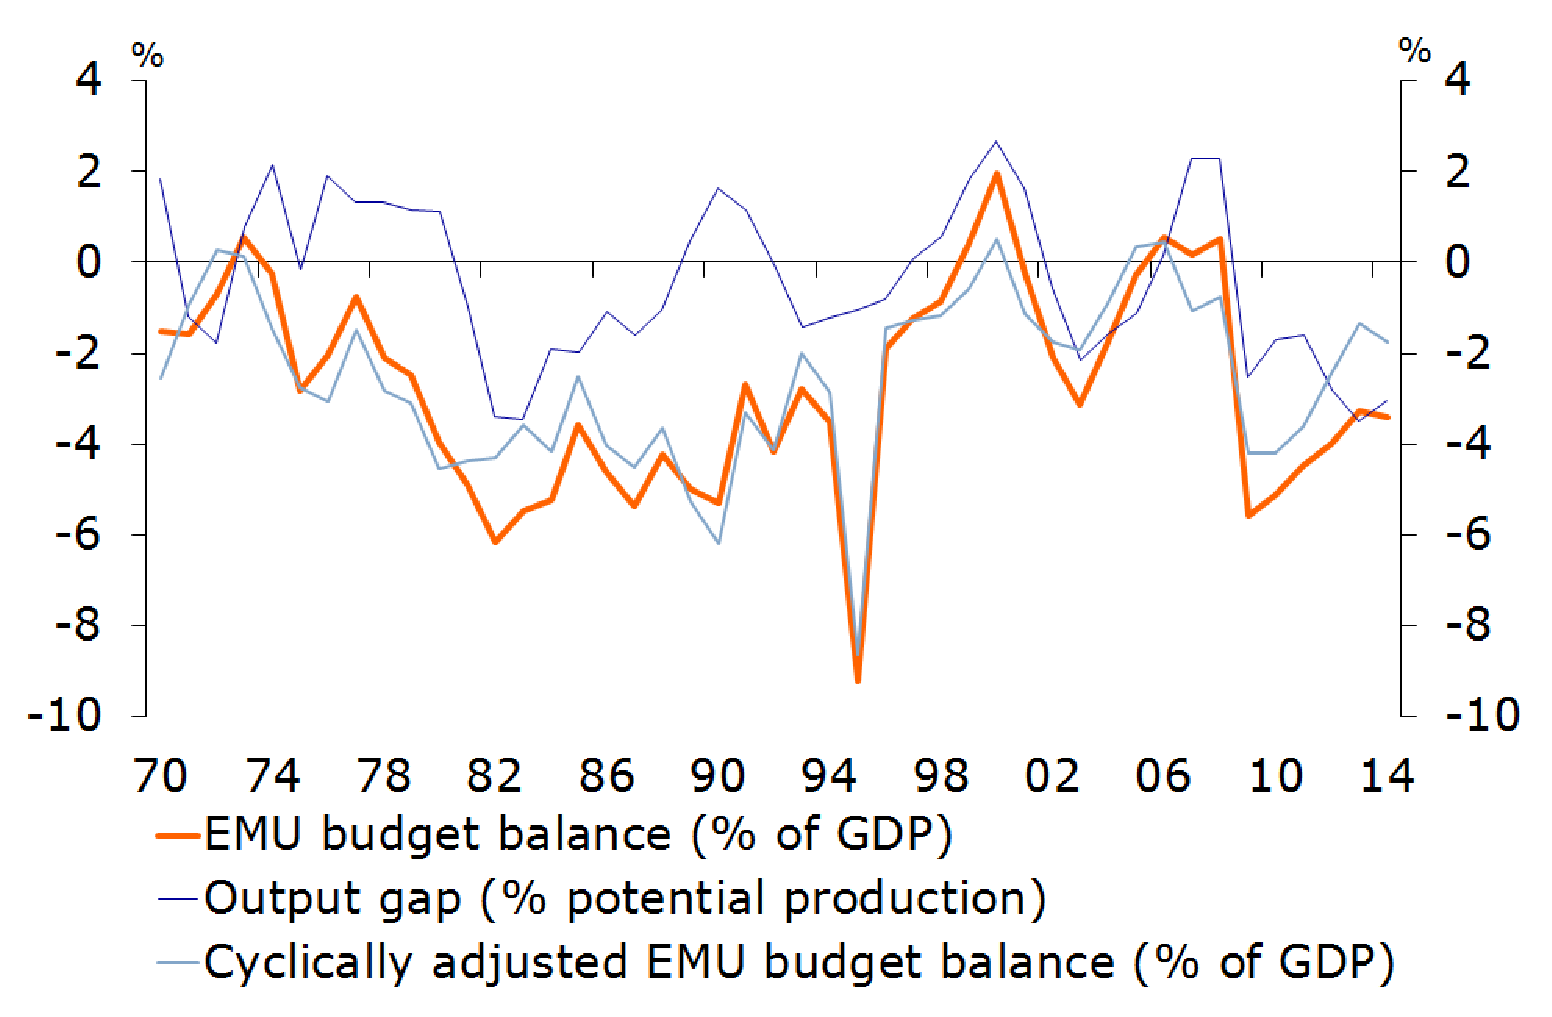
\includegraphics[scale=.3]{nl_budget}
  \caption{Actual and cyclically-adjusted budget balance along with the output gap for the Netherlands. Source: Rabobank}
  \label{fig:rabo}
\end{figure}
%--------------------------------------

%------------------------------------------------------------------------------
\section{Fiscal policy in the EU}
Although the EU member states have autonomy over their fiscal policy, one could imagine that fiscal policy has spillover effects generating externalities for other countries.\footnote{Business cycles are transmitted via imports and exports.} 
As such, it might be beneficial for the member states to coordinate their policy measures, at least to some extent. 
Which brings us back to the Economic and Monetary Union (EMU)
Among the 28 members of the European Union\marginnote{Likely to be 27 in the near future.} there is an agreement to facilitate and maintain the stability of the EMU.
Recall from the last lecture that for a country to join the EMU there were a number of entry conditions which included
\begin{itemize}
  \item Having a budget deficit no more than 3\% of GDP
  \item A public debt less then 60\% of GDP
\end{itemize}
But what are the rules when a country is already a member of the EMU?
An important pillar of the Maastricht Treaty was fiscal discipline and the rules concerning setting fiscal policy are set out
\begin{itemize}
  \item the Stability and Growth Pact (SGP)
  \item the Excessive Deficit Procedure (EDP)\marginnote{The EDP is part of the SGP (corrective arm) and was adopted in 1997 and meant to be strictly enforced, there have been some issues with this however. Currently 11 of 28 member states are subject to and EDP}
\end{itemize}

%------------------------------------------------------------------------------
% SGP
\subsection{The Stability and Growth Pact}
The Stability and Growth Pact (SGP) was established in 1997 to improve the coordination and monitoring of fiscal and other economic policies of the member state, and importantly to enforce the deficit and debt limits as established by the Maastricht Treaty. 
The main objective of the SGP is to ensure that EU member countries pursue sound public finances and coordinate their fiscal policies. 
The SGP has evolved over time along with EU's economic governance rules
\begin{itemize}
  \item 1998: Preventive rules of SGP enter into force
  \item 1999: Corrective rules of SGP enter into force
  \item 2005: Amendment to SGP for better consideration of national circumstances\footnote{Also added more economic rationale to the rules to be complied with.}
  \item 2011: Six pack added
  \item 2013: Two pack and Fiscal Compact added
  \item 2014: Review of SGP
  \item 2015: SGP flexibility; European Commission issuing guidance on how rules will be applied
\end{itemize}

The SGP as established in 1997 was based on three main elements
\begin{enumerate}
  \item Prevention
  \begin{itemize}
    \item Entered into force in 1998
    \item Each EU member state is set a budgetary target in order to bind the government to their commitment towards sound fiscal policy and coordination\marginnote{This is known as the  Medium-Term Budgetary Objective (MTO) which are updated every three years.}
    \item Budget deficit is defined in structural terms\footnote{This means that it takes into account the business cycle and filters out one-off or temporary measures.}
    \item The member state has to provide an annual budget outlining how to reach the targets, which is assessed by the European Commission and the EU governments\marginnote{Recall that these rules apply to both Eurozone countries and all other EU member states.}
  \end{itemize}
    
  \item Correction
  \begin{itemize}
    \item Entered into force in 1999
    \item This is where the Excessive Debt Procedure (EDP) enters into play
    \item The EDP ensures the correction of excessive budget deficits ($>3$\% of GDP) or public debt levels ($>60$\%)\marginnote{According to the European Commission public debt levels are excessive when it exceeds 60\% of GDP and does not diminish at an adequate rate of 5\% per year on average over the last three years}
    \item The EDP is a step-by-step procedure
  \end{itemize}

  \item Enforcement
  \begin{itemize}
    \item Sanctions may follow when countries fail to respect the preventive and corrective rules
    \item For Eurozone countries these could be fines
    \begin{itemize}
      \item 0.2\% of GDP, if they fail to abide by either the preventive or the corrective rules
      \item 0.5\% of GDP, if they repeatedly fail to abide by the corrective rules
    \end{itemize}
    \item For all member states the penalty could be suspension of commitments/payments of the structural and investment funds\marginnote{Strangely, the UK is excluded from these penalties. In general, one criticism is that the rules are hardly ever enforced on Germany and France, who were much in favour for the SGP.} 
  \end{itemize}
\end{enumerate}

%------------------------------------------------------------------------------
% SGP PLUS
\subsection{Adjustments to the Stability and Growth Pact}
Over the years some adjustments have been made to the SGP in order to make it more comprehensive, predictable, and efficient. 
Most importantly the economic governance rules were adjusted following the sovereign debt crisis with a set of new law known as the Six Pack
The Six Pack rules stipulate the following for EU goverments 

\begin{enumerate}
  \item Operate public accounting systems that comprehensively cover all areas of income and expenditure\marginnote{These must be subject to internal control and independent audits}
  \item Make the fiscal data publicly available (monthly basis for central and state governments, quarterly for local governments)
  \item Ensure their fiscal planning is based on realistic macroeconomic and budgetary forecasts, using the most up-to-date data
  \item Operate specific fiscal rules to help ensure the overall government budget complies with European rules
  \item Establish a credible, effective medium-term budgetary framework that includes a 3 year fiscal planning horizon
  \item Ensure consistency and coordination of all accounting rules and procedures across all areas of government activity
\end{enumerate}

The objective of this set of additional rules was to
\begin{itemize}
  \item Enhance marcoeconomic surveillance
  \item Improve procedures to address public deficits and other macroeconomic imbalances 
\end{itemize}

An additional set of rules were implemented in 2013 with the Two Pack which is a set of regulations that require member states to increase 
reporting frequency to enhance surveillance. 
In 2013 the EU also implemented a law called the Fiscal Compact which is basically a stricter interpretation of the SGP concerning the importance of the budgetary targets set out in the SGP's preventive arm.\footnote{I.e. the medium-term budgetary objectives. The Fiscal Compact is part of a larger treaty; Treaty on Stability, Coordination, and Governance. This treaty was signed by all member states except for Czechia, the United Kingdom, and Croatia (a recent new member).}

%------------------------------------------------------------------------------
% FISCAL COMPLIANCE
\section{Fiscal compliance}
\begin{figure}
  \caption{Development of budget deficit (\textit{top}) and public debt (\textit{bottom}) as percentage of GDP over time. Blue line indicates the average for 17 Eurozone member states, dotted horizontal line indicates the 3\% and 60\% criteria of the Maastricht Treaty repsectively. Data: Eurostat}
  \includegraphics[scale=.2]{budget_deficit}
  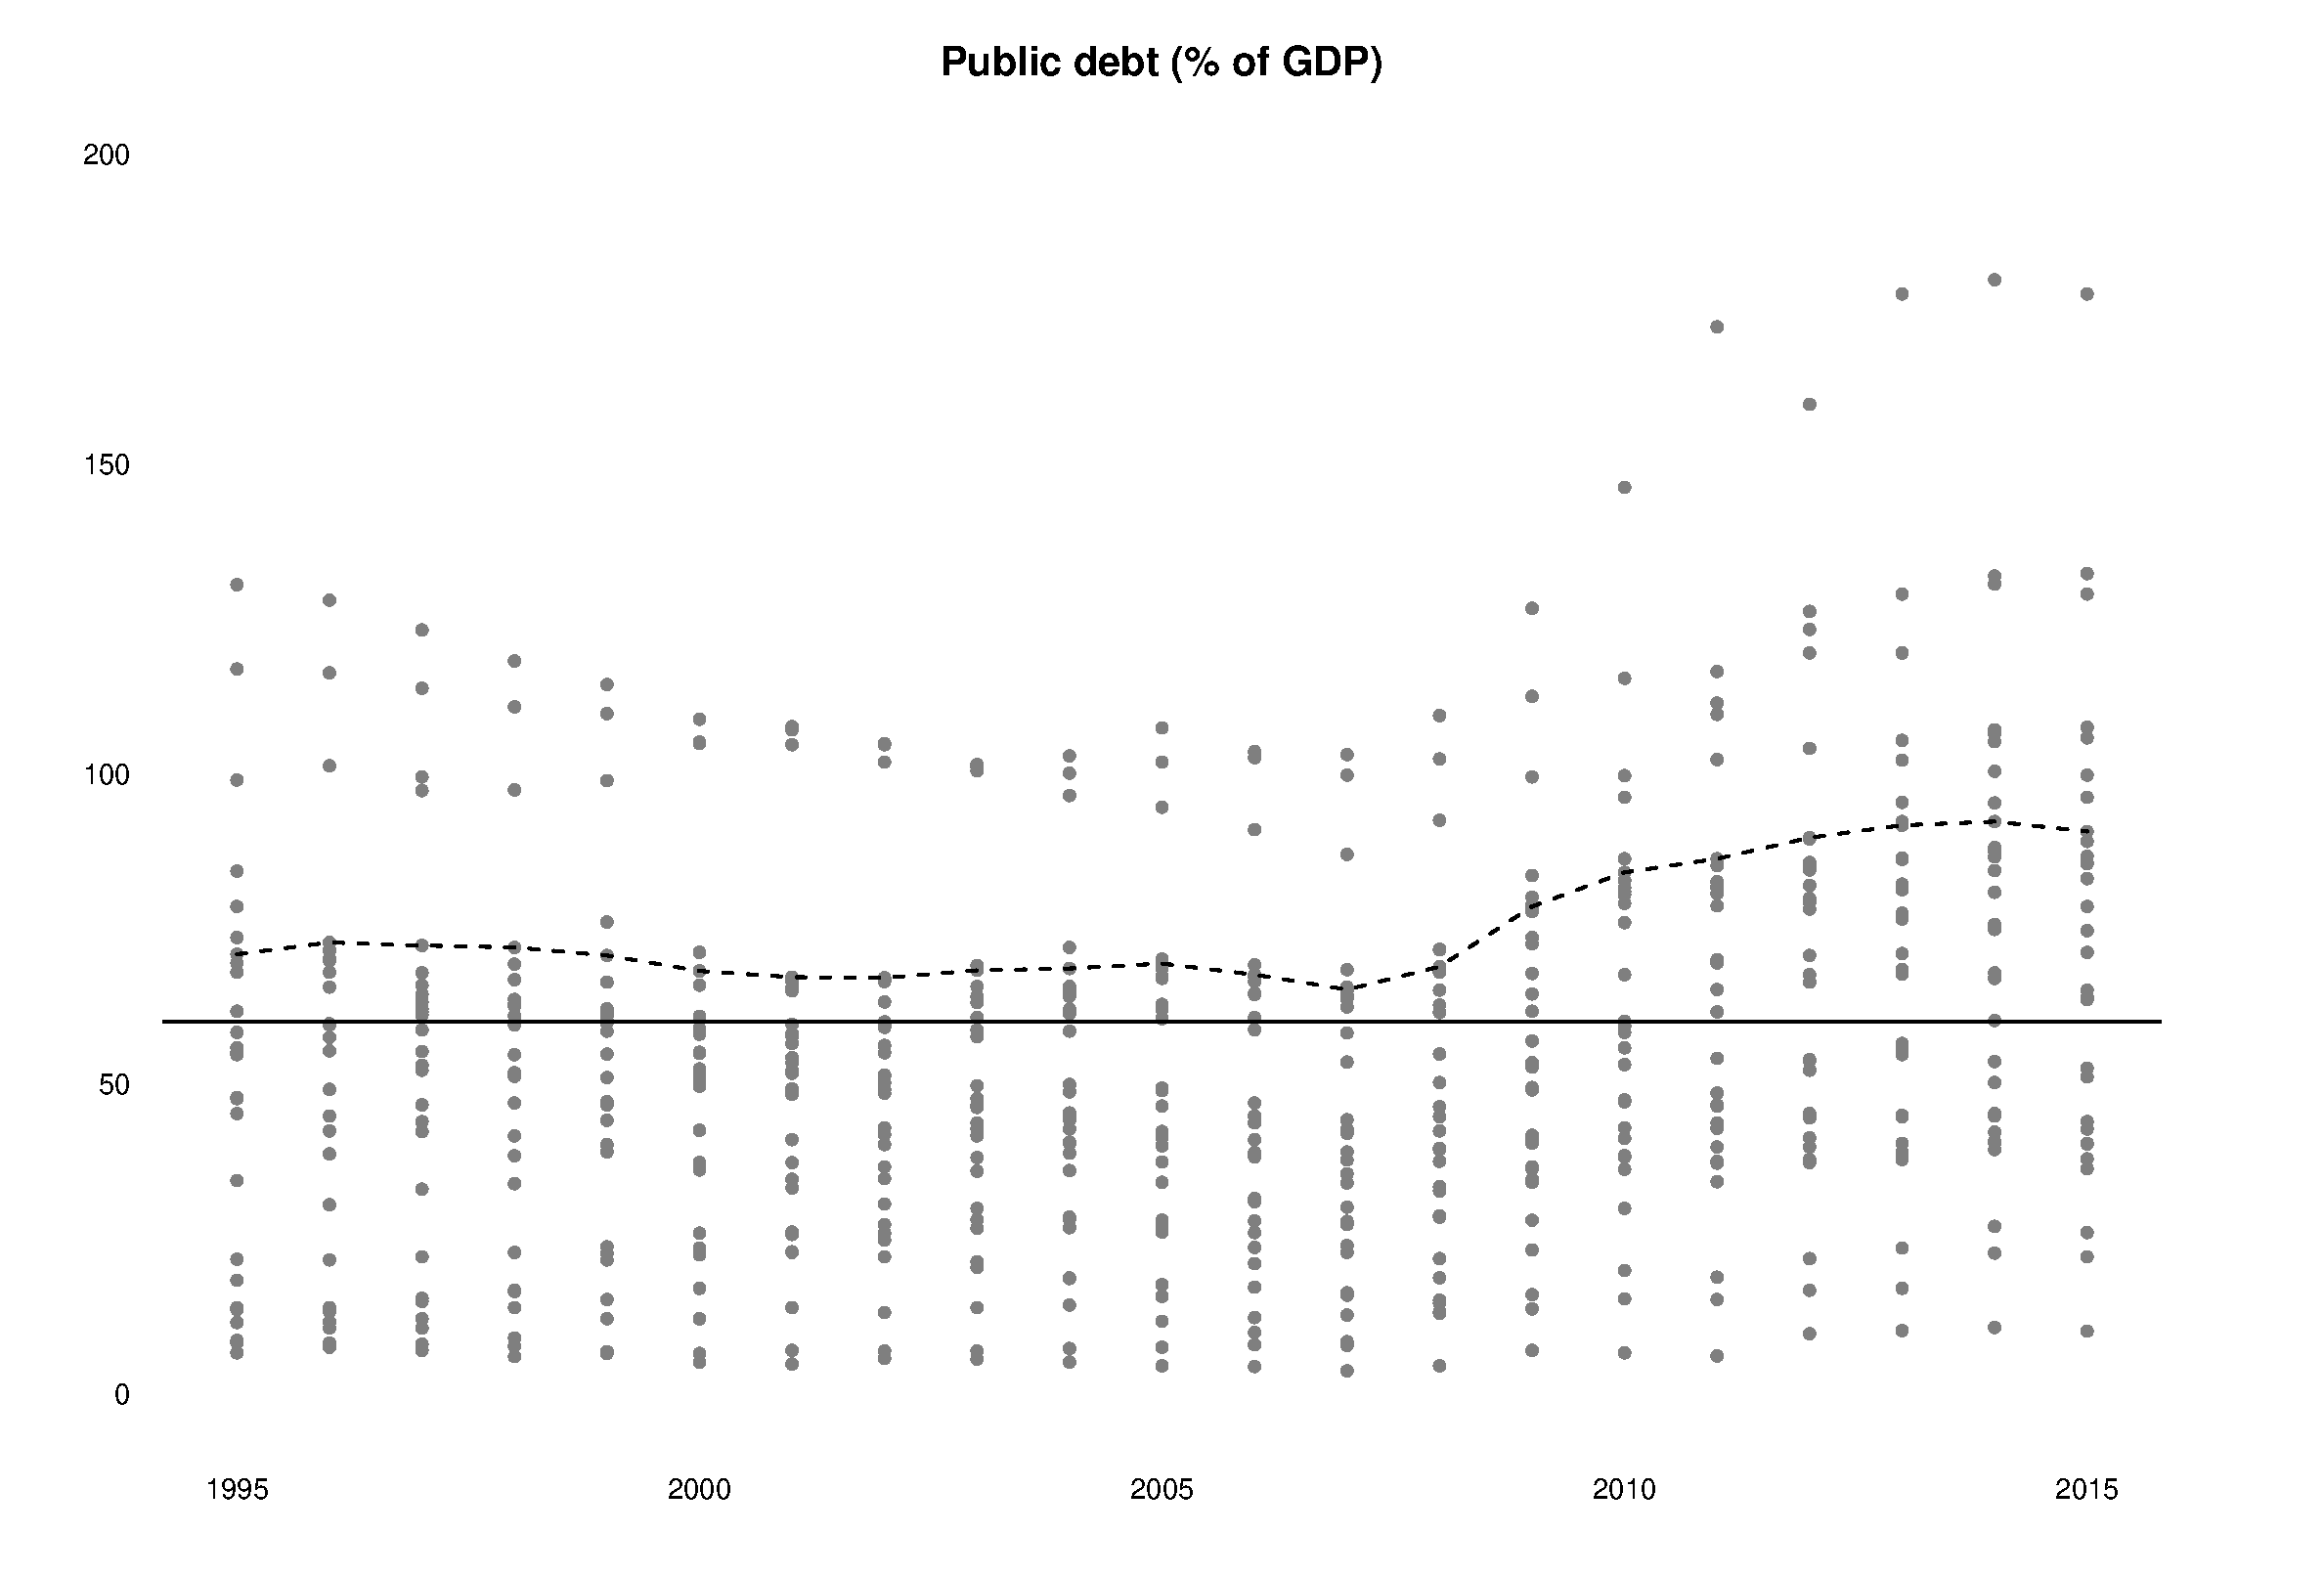
\includegraphics[scale=.2]{public_debt2}
\end{figure}

\begin{marginfigure}
  \caption{Average budget deficit and public debt during 2011-2015. Data: Eurostat}
  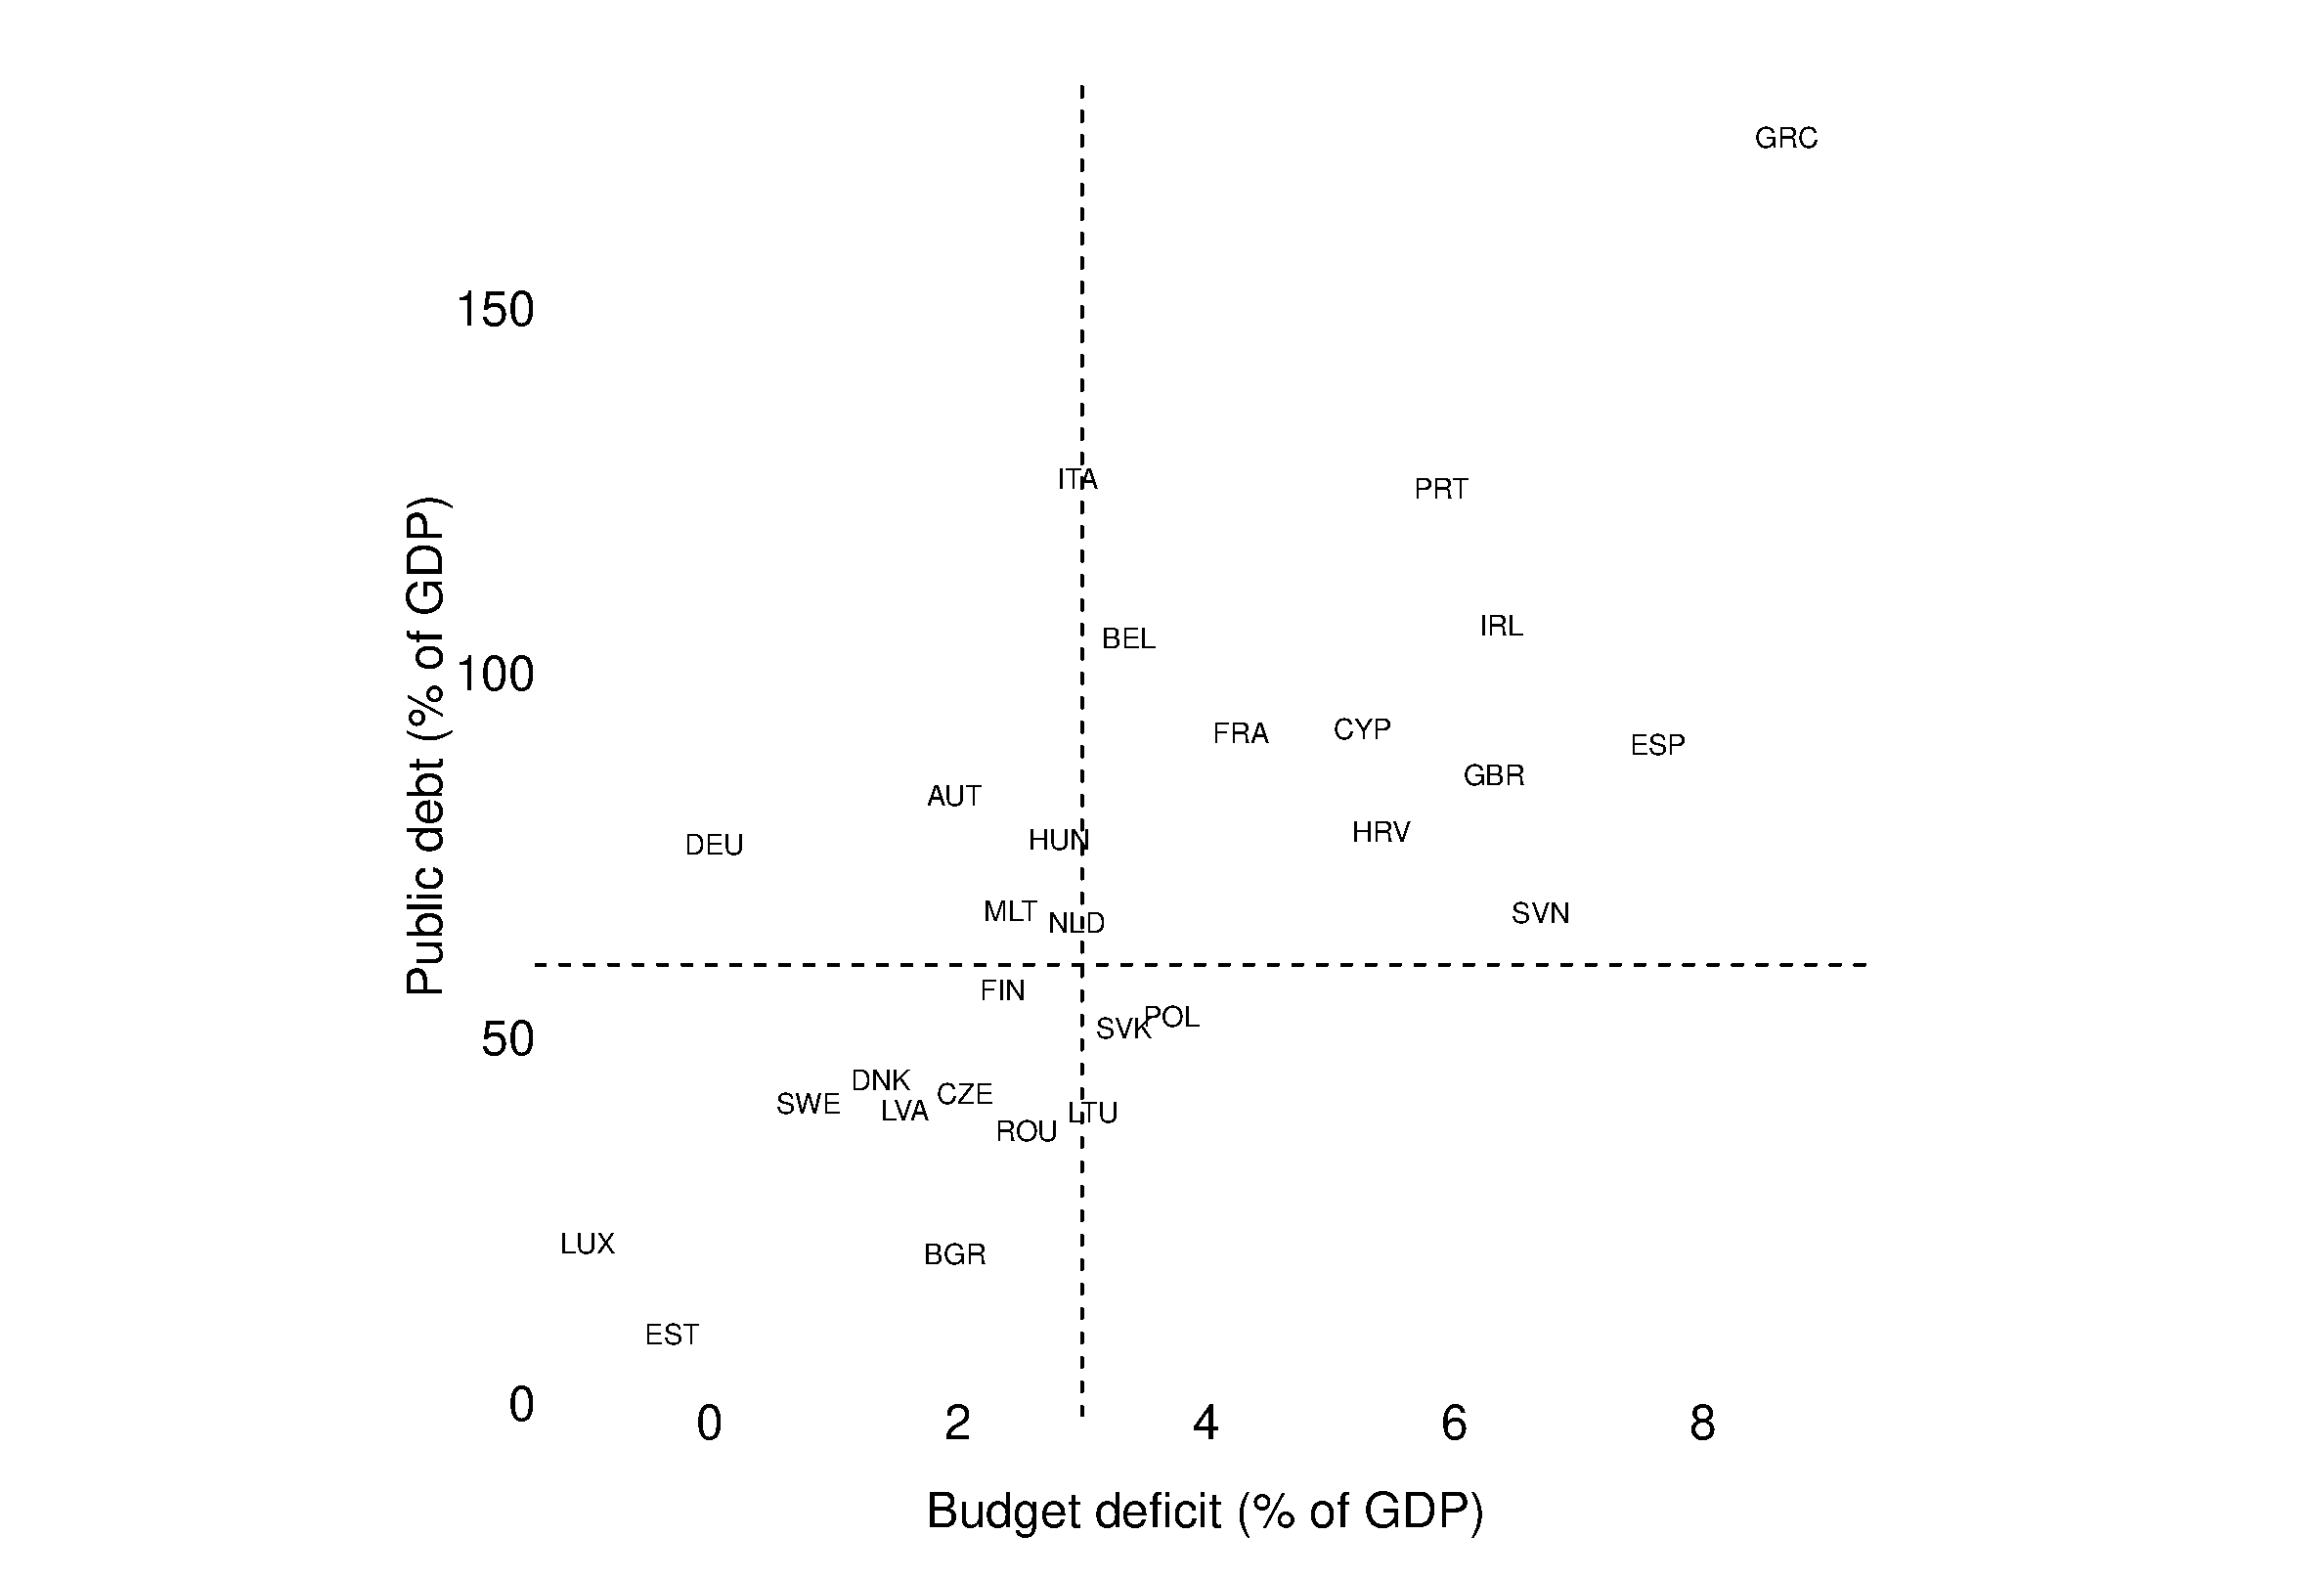
\includegraphics[scale=.1]{fiscal_compliance}  
\end{marginfigure}


%------------------------------------------------------------------------------
% EDP
\section{The Excessive Deficit Procedure}
The Excessive Debt Procedure is the corrective arm of the SGP.
This is a step-by-step procedure where the European Commission, using the data from Eurostat, examines the issue at hand and sets deadlines for the member country for which the procedure is started to reach the target level as defined in the MTO.\marginnote{So it is initiated when deficit exceeds 3\% of GDP or when debt exceed 60\% of GDP and is not sufficiently diminishing.} 
The procedure takes the following steps
\begin{enumerate}
  \item European Commission reports on whether to open the EDP
  \item The European Council decided whether an excessive deficit exists, and if so opens an EDP
  \begin{itemize}
    \item At this stage recommendations are made followed by deadlines and targets
    \item In some cases sanctions can be issues
  \end{itemize}
  \item The member state has 3-6 months to comply with the recommendations
  \item The Commission assesses if the member state has taken effective action and informs the council
  \begin{itemize}
    \item Member state has taken effective action and the targets are met $\rightarrow$ Council takes note
    \item Member state has taken action but targets aren't met $\rightarrow$ council revises recommendation, extend deadlines $\rightarrow$ Back to 3 
    \item Member state has not taken effective action $\rightarrow$ Council gives new recommendations etc. $\rightarrow$ Back to 3
    \item In the case the the member state is also part of the Eurozone, additional sanctions follow when no effective action is taken
  \end{itemize}
  \item European Commission proposes EDP abrogation, Council takes final decision
\end{enumerate}
%------------------------------------------------------------------------------
\clearpage
% CALCULATING MTO
\section{Background: Calculating the Medium-Term Budgetary Objective}
\marginnote{Taken from \href{http://ec.europa.eu/economy_finance/publications/european_economy/2013/pdf/ee-2013-4.pdf}{Report on Public Finances in EMU 2013}}
The Medium-Term Budgetary Objectives are calculated taking into account the fluctuations in the business cycle, specifically the reaction of a member state's budget to these fluctuations. 
The final MTO is based on a number of components.
Concerning the budget deficit, for each country a MTO is calculated that ensures a safety margin, called the minimum benchmark, which accounts for past volatility and the sensitivity of the budget to fluctuation in output.\footnote{I.e. a country that experiences a lot of volatility and where the budget is very sensitive to fluctuation in the business cycle will need a more demanding MTO to ensure that they stay within the 3\% limit. } 
The minimum benchmark MTO is calcualted the following way
\begin{align*}
  MTO^{MB} = -3 -\epsilon ROG
\end{align*}

In this formula $\epsilon$ is the semi-elasticity of the budget to the output gap and $ROG$ stands for the representative output gap. 
The $ROG$ accounts for the fact that different countries face different magnitudes of the business cycle and is calculated as
\begin{align*}
  ROG = \frac{N_i}{(N_t+N_i)}P_{5\%}country + \frac{N_t}{(N_t+N_i)}P_{5\%}(EU27)
\end{align*}

Here $P_{5\%}$ represents the 5\% percentile of the distribution of the output gap series of either the country or all member states. 
$N_i$ and $N_t$ stand for the country-specific observations available, where $t$ is, data permitting, set to 25 years. 
Moving on to public debt, for each member state a minimum value for the MTO is set that helps the country to converge to a prudent debt level (60\% of GDP) and is calculated accounting for implicit liabilities and debt (ILD) following
\begin{align*}
  MTO^{ILD}= Balance_{debt-stabilizing(60 \% of GDP)} + \alpha AgeingCosts + Effort_{debt\;reduction}
\end{align*}

The three terms on the right hand side of the equation represent (in order)
\begin{enumerate}
  \item The budget balance that would stabilise the debt ratio at 60\% of GDP\footnote{This is calculated as the product of 60\% with the forecast  average  nominal  growth  over  the  next  50 years}
  \item An adjustment required to cover a fraction of the present value of the projected increase in age-related expenditure\footnote{$\alpha=33\%$}
  \item A supplementary debt-reduction effort for countries with debt above 60\% of GDP\footnote{This is 0.2\% if debt is above 60\% and 1.4\% when the debt reaches 110\%.}
\end{enumerate}

Besides these two MTOs accounting for the main criteria set out in the SGP there is an extra MTO for Euro area and ERM2 member states which is
\begin{align*}
  MTO^{Euro/ERM2}=-1\% GDP
\end{align*}

All the MTOs are then combined to compute a country-specific lower bound according to
\begin{align*}
  MTO = max (MTO^{ILD},MTO^{MB},MTO^{Euro/ERM2})
\end{align*}










\end{document}
